\section{Educational Activities}
\label{sec:approach}
% Course Development
% BPC - Mentoring/Recruitment - Leverage existing recruiting mechanisms, mentoring participant costs

\begin{wrapfigure}{r}{.5\textwidth}
\centerline{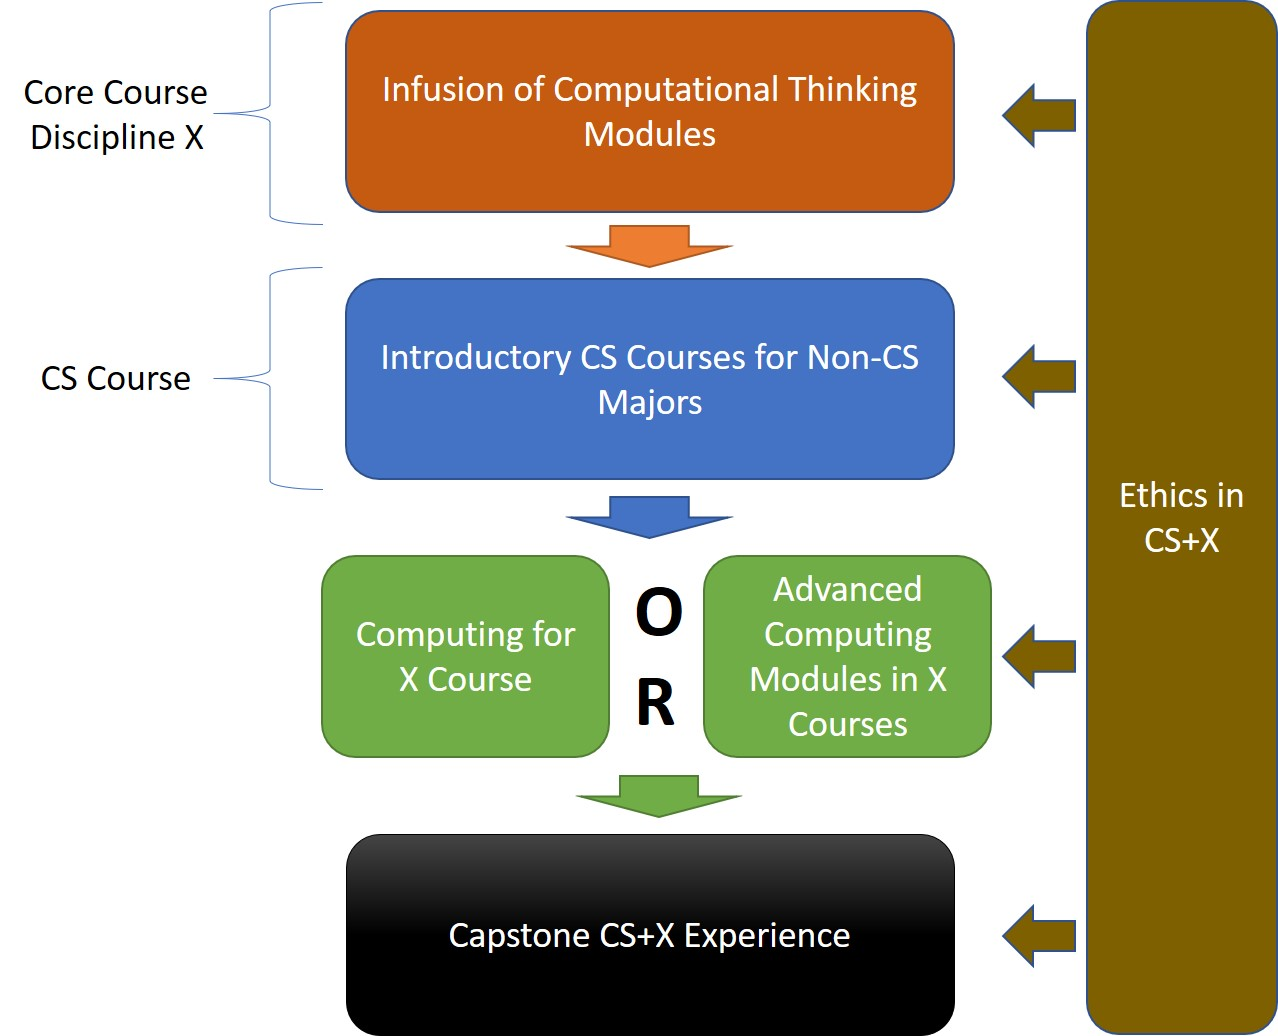
\includegraphics[width=.45\textwidth]{Picture1.jpg}}
\caption{Progression Flow of Educational Components}
\label{fig:structure}
\end{wrapfigure}
The overall structure of the educational program we propose for integrating computing education with diverse disciplines is based on four flexible curricular elements shown in Figure~\ref{fig:structure}. These elements are designed to be customized to the needs of the  discipline into which they are being integrated and the students of that discipline. Ethics elements focused on computing problems relevant to the discipline into which computing instruction will be developed. Finally, each element is augmented with cross-cutting student mentoring and support programs designed to increase student success and retention. 

The remainder of this section overviews the proposed curricular elements, describes how ethics training will be integrated, and discusses the student mentoring and support programs. Pilot integration of this approach into multiple disciplines are presented in section~\ref{sec:pilots}.

\subsection{Curricular Elements}
\subsubsection{Introductory Course Modules}

\paragraph{Goals:} The goal of this educational component is to provide initial exposure to computational thinking (CT). This component will achieve the following specific goals: {\bf (1)} Provide an initial exposure and preliminary preparation in the core concepts of computing (e.g., algorithmic thinking); 
{\bf (2)} Build engagement and gain interest in computing for an audience of diverse non-CS students.
Placing CT in the context of a domain benefits the teaching of computing by simplifying the
illustration of CT, anchors the principles and practices of CT within the target domain, and demonstrates the relevance of computing to topics that are relevant and appealing to the students.
Infusing CT into a target discipline has also benefits the discipline by  facilitating inquiry-based learning, exploratory analysis and providing structure to the
domain \cite{ep71,ep150}.  CT enables reasoning at different levels of abstraction, and emphasizes the transition from
using information to creating knowledge.

\paragraph{Instructional Approach:}
The instructional approach adopted in this component consists of the development and deployment of course modules in the context of selected non-CS courses. The emphasis will be in core/required courses, typically at the sophomore level; this will ensure an  audience committed to the target discipline, provide clear ties of computing to the foundations of the target non-CS discipline. 
%and allow students' exposure to computing sufficiently early in their academic pathway.
The  process will be realized by modifying lectures and class activities to emphasize the use of computing concepts to explain core content of the target non-CS discipline. The redesign of the modules for each course will be realized by a team composed of the class teacher, a CS faculty and a CS student assistant.  

One of the key underpinnings of this project
is that most disciplines  provide ample opportunities to demonstrate 
a comprehensive set of foundational computing concepts,  ranging from algorithms (e.g., the procedure to obtain and execute a warrant is often  described using an informal UML structure), to data (e.g., categorizing words based on
etymology), to abstraction (e.g.., identifying irrelevant
parts of a paragraph, a task in ACT English college
readiness standards, commonly explained by implicitly
building a conceptual network and reasoning about
reachability), to rules (e.g., capturing the syllogisms in
an opinion paper), to systems (e.g., the description of
blocking in stage productions \cite{ep115}).

%The modules will provide a gradual shift from: {\bf (i)} 
%\emph{passive illustration} of concepts (e.g., a graph
%representation of causal dependencies in a story) to 
%{\bf (ii)} 
%\emph{interaction} (e.g., explore associations between
%sentences and abstracted causal dependencies) to 
%{\bf (iii)} 
%\emph{question-answer} (e.g., given a set of assumptions,
%draw conclusions using the causal structure) to 
%{\bf (iv)} \emph{computation} (e.g., design a sequence of steps to validate
%if the conclusions by an author are supported by his arguments).

\paragraph{Curricular Integration:}
Consider a sequence of modules that to introduce different concepts of computational thinking in the context of a basic Molecular Biology course:
\begin{tightenumerate}
\item \emph{Passive Illustration:} computer animation  for protein structure and protein-protein docking; 
\item \emph{Interactive Illustration:} Interaction to select segments of primary sequence and highlight the corresponding 3D substructure (e.g., find the helix in the primary sequence);
\item \emph{Question-Answer:} Visual manipulation of a 3D molecule to recognize (by visual comparison against a table of 2D images of amino acids) the displayed amino acid;
\item \emph{Problem Solving:} Write an iterative algorithm to run a structural alignment program to find a mystery protein in a collection of known proteins.
\end{tightenumerate}
The modules follow a  progression that moves from the use of computing to illustrate content of the course to the actual development of algorithms.

\subsubsection{Core Computing Class Modules}
\paragraph{Goals:} Introductory computing courses will provide  students the tools to further \emph{expose} students to computing techniques and teach them to \emph{use} these techniques to solve problems in multiple disciplines.

\paragraph{Structure:} We will build upon existing introductory CS courses at the 3 institutions (e.g. CS108 NM CS for All at UNM, CS105 Introductory Programming, a pre-majors course at UNM; CS 111, a pre-major CS course, and CS171G General Education at NMSU; CSE107 Introduction to Programming at NMT.) These existing courses have already taught thousands of students who are non-CS majors or pre-majors. We will emphasize teaching modules that teach general computing knowledge (abstraction,problem decomposition, iteration, conditional statements) as well as modeling and simulation and data analysis tools that are useful in our disciplinary domains.

\paragraph{Curricular Integration:}
We will not develop new introductory non-major courses, but instead will shift the focus of some introductory courses to more directly address needs of students from the target disciplines.c We will survey students to determine their intended major and assess whether introductory courses are meeting the needs of non-CS majors.

\subsubsection{Expertise-Building Disciplinary Computing Course Strands}
\paragraph{Goals:} The goal of this educational element is to provide a set of extended instructional modules (strands) to teach students mastery the use of computing techniques in their discipline. For students who have completed core computer science classes and have programming experience suitable for their disciplinary need, these strands will provide skills to use computer science techniques for solving common disciplinary computer- and/or data-intensive problems. 

\paragraph{Structure:} We will develop a set of four-week strands that cover key computer science topic areas through the lens of problems in a specific discipline. Because of the data-centric nature of most of the disciplines on which we focus, we plan to initially focus on course modules that teach fundamentals of data structures, algorithm analysis, object-oriented programming, parallel programming, data analysis, and computing ethics through discipline-specific examples. In addition, we plan to design the modules so that the four weeks of content can be split into overlapping two or tree week modules that can be used in successive classes in a sequence to provide students multiple exposures to each topic. The exact topics, length, and structure of each strand to facilitate customization will be determined during pilot development (Section~\ref{sec:pilots}) and refined using our proposed assessment and evaluation (Section~\ref{sec:assessment}) framework.

\paragraph{Curricular Integration:} In most cases we expect these strands to be integrated into computing-enhanced disciplinary research methods classes. As mentions above, our default structure will be to split each four-week strand into two overlapping three-week modules. We anticipate that four four-week strands would be split across three research methods classes in the UNM sociology/criminology program, for example starting with the SOC380 Introduction to Research Methods and continuing in SOC381 Sociological Data Analysis
 and SOC481 Data Analysis. This will provide each class approximately 6 weeks of relevant computing education to integrate into the existing curriculum. In other cases, however, we will research combining 4 strands into a single class, for example to create a single Health Informatics course at NMSU. 

\subsubsection{Capstone X + CS Projects}

\paragraph{Goals:} The goal of this educational element is to provide program participants with a final integrative project to combines their disciplinary knowledge with their fully-developed computer science expertise. 

\paragraph{Structure:} For this element, we will develop general outlines of projects or disciplinary project approaches that students can, with guidance from a course instructor, use to create a full-formed final project. In each discipline, general project outlines will describe methods for using state-of-the-art computing techniques in different disciplinary areas, for example general classes of machine learning techniques for different classes of disciplinary data or general computational modeling techniques relevant to disciplinary problems.

\paragraph{Curricular Integration:}
These project outlines will be used by students in either disciplinary capstone design classes or through a senior-level computer science classes open to CS-literate disciplinary practitioners. Both types of classes are common at the all three institutions. Science and engineering disciplines, for example, often include single- or multi-semester senior design seminars for their students. In addition, all three institution's computer science departments also offer senior-level project-based ``Introduction to Big Data'' classes open to CS-literate students from other disciplines and UNM also teaches a similar senior-level ``Scientific Computing'' class. In the former case, project information would provide students suggestions about how to integrate computing into discipline capstone projects. In the later case, the outline would point students to the kinds of disciplinary projects to which the big data or scientific computing the students are learning could be applied.


%\For At NMT, the capstone projects will be designed in such a way that they are determined and completed through the course of multiple semesters. Students with Psychology and Business Technology \& Management majors will identify and develop their capstone project ideas while taking expertise-building disciplinary computing course strands described in the previous subsection, and they will complete their capstone project in a Senior Design Clinic where they typically present their findings to peers and faculty members at the end of the Clinic course. Students will be supervised by both computer science and relevant discipline faculty members.

%\textcolor{blue}{[From Huiping], AT NMSU, the capstone project will allow the students to work on a criminal justice/nursing problem by utilizing DA and Information System techniques. The students will be advised by two faculty, one from computer science and the other from criminal justice/nursing.
%}

\subsection{Ethics Training Integration}
Ethical considerations are a critical component in the educational process~\cite{stahl}. Previous studies have argued the importance of integrating ethics throughout computer science and engineering curricula rather than in standalone courses~\cite{newberry,yale-weltz}. Incorporating ethics across the curriculum helps students understand the link between the practice in the field and its positive and negative impacts and also see ethical considerations as part of computer science, rather than an add-on~\cite{newberry, pantazidou, yale-weltz}. The application of computing technologies in different disciplines, despite their significant benefits, involves the possibilities for wrongdoing, e.g., biased algorithms and record tracking systems that influence negatively the lives of minorities and the poor and treat them unjustly~\cite{oneil}. This necessitates the development of professionals who not only possess computational skills, but also are aware of ethical and social implications of the systems they will design or use~\cite{connolly,stahl}.

We will develop a number of ethics modules that will be incorporated into existing courses within partner programs that follow the Association for Computing Machinery (ACM) Code of Ethics and Professional Conduct~\cite{acm-ethics}. In addition to developing modules to address computer science issues relevant to specific disciplines covered in the proposed courses, we will use of case-based discussions to engage students in the process of ethical decision making and raise their awareness about the ethical implications of computing practice in their future professional lives. Based on the content of each CS course, a we will develop a real-world scenario along with a discussion protocol, deployable in an online or face-to-face format, in which students will answer questions and comment on their peers’ reasoning and arguments. These discussions will not only make students aware of the ethical issues within the field, but also will help them see the ethical scenarios from different perspectives and  realize the complexity of the ethical issues and the importance of addressing them properly. In addition, course instructor(s) will gain insights into the student ideas and ethical understanding which can be used in developing interventions to improve instruction for future offerings of the course.

\subsection{Student Support Activities}
\label{sec:framework:support}

The proposed project will provide student supports that help them succeed in the proposed courses and capstone project, including faculty advising, tutoring, and peer mentoring. Students will be initially advised by faculty members to conduct a self-assessment of their interest, strength and deficiency for the proposed computing classes. Then students will develop a course plan toward their capstone project with the faculty members who will monitor their progress and provide additional assistance for their success with tutoring and peer mentoring. These activities will leverage existing programs provided by CAHSI INCLUDES, which focuses on the promoting computer science education at primarily HSIs.


As the CAHSI INCLUDES southwest region’s lead institution, New Mexico State University will serve an integral role in providing student support services for this project, coordinating with existing student support programs of UNM and NMT. 
The specific activities that we propose to introduce in  support of the students in the NMIX+CS program are primarily constructed on the themes of 
 \emph{teamwork} and \emph{mentoring}---as instruments to create leadership and professional
skills, and inspire a sense of accountability. These are critical factors to promote the success of
undergraduate students in technical fields, especially Hispanic students. Two specific CAHSI practices that we will adopt are Peer-Led Team Learning (PLTL) and the Affinity Research Group (ARG) model. 

The PLTL model of instruction will provide an active learning experience for students in the new courses introduced by this project, by engaging peer mentors
in the role of discussion leaders, who coordinate out-of-class team learning sessions (e.g., problem
solving workshops). PLTL provides leadership building activities for the team leaders and dynamic learning experiences for students in the course, essential to improve retention and advancement. This mentoring component will be critical as students from the target disciplines start navigating the more in-depth CS content (in the core computing class and the expertise-building disciplinary strands). 

The ARG model will be introduced to enhance success and learning in the capstone component. ARG \cite{arg1,arg2} is a comprehensive model for creating and maintaining dynamic, productive, and inclusive research groups. Application of the model entails the deliberate design of research groups whose members share a common purpose (an affinity) and it emphasizes the conscious development of students’ disciplinary knowledge, research abilities, and team
skills, as well as their sense of professional identity. ARG is structured to engage diverse groups of students, encouraging accountability and participation, capitalizing on the strengths of individual students and developing strategies to strengthen their weaker areas. This will be particularly important as we bring together in the capstone experience students with potentially different levels of computing competency and expertise in the target discipline. ARG has been shown to be effective in building a culture of research and a profound sense of mastery and self-efficacy.


CAHSI will utilize members of the CAHSI Club and Young Women in Computing (YWiC) to serve as peer mentors. Additionally, CAHSI scholars and YWiC will actively recruit students and perform outreach with the following academic specific-programs to support students: Sigma Theta Tau-Pi Omega Nursing Honor Society, Student Nursing Association, Nursing Advising Center, Alpha Phi Sigma Criminal Justice Society, and the Criminal Justice Mentoring Center. The three institutions will also provide additional assistance to mentor, advise, and tutor students through other existing resources, such as American Indian Program, Black Programs, Campus Tutoring Services, central offices for academic advising and student support, Chicano Programs, Military and Veterans Programs, TRiO Programs, and TRiO STEM-H Student Support Services. 